
The interconnection network simulator, Booksim, was created by the Concurrent VLSI Architecture group (CVA) at Stanford to study network on chip and large scale computer systems. The simulator allows for a wide range of user customizations when constructing a network. The simulator supports a variety of network topologies, router micro-architectures, routing algorithms, traffic pattern, and simulation modes. The priority of the simulator is  to guarantee the correctness and accuracy of simulation, and as a result the simulator is implemented in a cycle-accurate fashion. Booksim has been used to generate results for many research publications \cite{cdragon,KimISCA07,PPIN}. 
\subsection{Simulator Organization}
Booksim is written in C++ and dynamically allocates a hierarchy of objects to represent the user specified network. Figure~\ref{fig:simulator} shows the anatomy of the simulator at runtime. At the core of every network simulation is a collection of router and channel objects which forms the framework of a network. Each channel acts as a FIFO with a reader and a writer router object. The router objects contain all the data structure and operations necessary to route packets through the network. Similar to networks in real life, routers are mostly isolated from each other and can only communicate through channels or simple global signals. As a result, the operations of individual routers are almost completely independent of other routers in the network. Surrounding the core network framework is the traffic manager which acts as an interface between the user tests and the underlying network. It handles the injection and ejection of traffic as well as gathering simulations statistics for the user. \\
~\\
\begin{figure}[h]
\centering
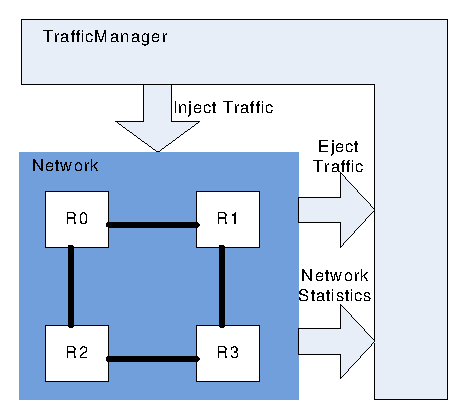
\includegraphics[width=3in]{simulator.eps}
\caption{Simulator organization: Network is composed of routers and channels and simulations are run through the traffic manager. }
\label{fig:simulator}
\end{figure}
Figure~\ref{fig:runtime} diagrams the runtime steps of the simulator. At the highest level is the network cycle loop. Each iteration of this loop represents a cycle in the network. Within each network cycle, several steps occurs to advance the state of the network. At each step, the simulator loops through all the routers in the network to perform a specific function. As mentioned previously the operation of routers are mostly independent of each other. Therefore, there are no dependencies between each iterations of these loops. Channels are the only source of sharing between the routers 
\begin{figure}[h]
\centering
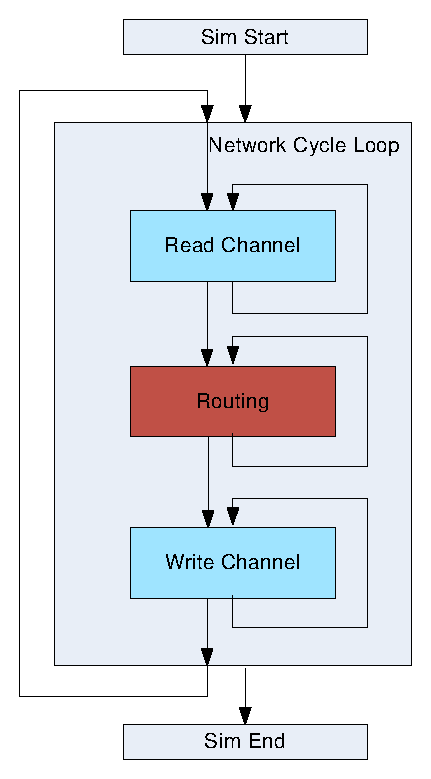
\includegraphics[width=3in]{runtime.eps}
\caption{Simulator runtime diagram. The number of iterations of the outer loop is equal to the number of simulated cycles. The number of iterations of each of the inner loops is equal the number of routers in the network.}
\label{fig:runtime}
\end{figure}
\subsection{Simulator Performance}
The simulator was originally designed for studying numerous aspects of small to medium sized interconnection networks (less than 100 network nodes). Nearly every aspect of the network is customizable and has been modeled in detail. Performance has not been a concern. However, the group's recent project involves simulating the dragonfly network \cite{cdragon}, which can easily grow to thousands or tens of thousands of nodes. Due to the organization of the simulator, the simulation runtime grows linearly with the number of network nodes and simulation time. A typical simulation of the dragonfly network involves running a networks with 10K nodes for at least 10K cycles to capture the network's steady state. Under the current simulator, this takes about 25 minutes. To generate an accurate latency-throughput plot of the network requires about 10 simulations. Furthermore, to see the effect of changes to a particular aspect of the network requires generating a latency-throughput plot each time. Such long simulation time increase the turn around time for research and limits the number of experiments that can be run reasonably. Currently, the group utilizes program level parallelism by running multiple simulations simultaneously on the cluster. But they are still limited by the runtime of each simulation.

Previously we have profiled the simulator to determine the program characteristics and hotspots. The program is composed of mostly integer operations. The only sources of floating calculation are for random packet generation and statistics collection. The program is control flow intensive: there are numerous branches inside of long running loops to determine the flow of packets and state of the routers. The program is also relatively memory demanding, since each network component is created as an object and network packets objects are dynamically allocated and deallocated as they enter and exit the network. In the typical dragonfly network modeled with realistic channel latencies, there is potentially hundreds of thousands of packets in flight simultaneously. Runtime profiling shows that 95\% of program time is spent in the routing step in figure~\ref{fig:runtime}. 

